% Chapter 1: Introduction to Time Series Analysis
% Harvard-quality academic presentation
% Bachelor program, Bucharest University of Economic Studies

\documentclass[9pt, aspectratio=169, t]{beamer}

% Ensure content fits on slides
\setbeamersize{text margin left=8mm, text margin right=8mm}

%=============================================================================
% THEME AND STYLE CONFIGURATION
%=============================================================================
\usetheme{Madrid}
\usecolortheme{seahorse}

% Professional Color Palette
\definecolor{MainBlue}{RGB}{26, 58, 110}
\definecolor{AccentBlue}{RGB}{42, 82, 140}
\definecolor{IDAred}{RGB}{220, 53, 69}
\definecolor{DarkGray}{RGB}{51, 51, 51}
\definecolor{MediumGray}{RGB}{128, 128, 128}
\definecolor{LightGray}{RGB}{248, 248, 248}
\definecolor{VeryLightGray}{RGB}{235, 235, 235}
\definecolor{Crimson}{RGB}{220, 53, 69}
\definecolor{Forest}{RGB}{46, 125, 50}
\definecolor{Amber}{RGB}{181, 133, 63}
\definecolor{Orange}{RGB}{230, 126, 34}
\definecolor{HarvardCrimson}{RGB}{165, 28, 48}

\setbeamercolor{palette primary}{bg=MainBlue, fg=white}
\setbeamercolor{palette secondary}{bg=MainBlue!85, fg=white}
\setbeamercolor{palette tertiary}{bg=MainBlue!70, fg=white}
\setbeamercolor{structure}{fg=MainBlue}
\setbeamercolor{title}{fg=MainBlue}
\setbeamercolor{frametitle}{fg=MainBlue, bg=white}
\setbeamercolor{block title}{bg=MainBlue, fg=white}
\setbeamercolor{block body}{bg=VeryLightGray, fg=DarkGray}
\setbeamercolor{block title alerted}{bg=Crimson, fg=white}
\setbeamercolor{block body alerted}{bg=Crimson!8, fg=DarkGray}
\setbeamercolor{block title example}{bg=Forest, fg=white}
\setbeamercolor{block body example}{bg=Forest!8, fg=DarkGray}
\setbeamercolor{item}{fg=MainBlue}

\setbeamertemplate{navigation symbols}{}

\setbeamertemplate{footline}{
    \leavevmode%
    \hbox{%
        \begin{beamercolorbox}[wd=.333333\paperwidth,ht=2.5ex,dp=1ex,center]{author in head/foot}%
            \usebeamerfont{author in head/foot}\insertshortauthor
        \end{beamercolorbox}%
        \begin{beamercolorbox}[wd=.333333\paperwidth,ht=2.5ex,dp=1ex,center]{title in head/foot}%
            \usebeamerfont{title in head/foot}\insertshorttitle
        \end{beamercolorbox}%
        \begin{beamercolorbox}[wd=.333333\paperwidth,ht=2.5ex,dp=1ex,right]{date in head/foot}%
            \usebeamerfont{date in head/foot}\insertshortdate{}\hspace*{2em}
            \insertframenumber{} / \inserttotalframenumber\hspace*{2ex}
        \end{beamercolorbox}}%
    \vskip0pt%
}

%=============================================================================
% PACKAGES
%=============================================================================
\usepackage[utf8]{inputenc}
\usepackage[T1]{fontenc}
\usepackage{amsmath, amssymb, amsthm}
\usepackage{mathtools}
\usepackage{bm}
\usepackage{tikz}
\usetikzlibrary{arrows.meta, positioning, shapes, calc, decorations.pathreplacing}
\usepackage{booktabs}
\usepackage{multirow}
\usepackage{array}
\usepackage{graphicx}
\usepackage{hyperref}
\usepackage{colortbl}
\hypersetup{colorlinks=false, pdfborder={0 0 0}}
\graphicspath{{../logos/}{../charts/}}

%=============================================================================
% THEOREM ENVIRONMENTS
%=============================================================================
\theoremstyle{definition}
\setbeamertemplate{theorems}[numbered]
\newtheorem{defn}{Definition}
\newtheorem{thm}{Theorem}
\newtheorem{prop}{Proposition}
\newtheorem{rmk}{Remark}

%=============================================================================
% CUSTOM COMMANDS
%=============================================================================
\newcommand{\E}{\mathbb{E}}
\newcommand{\Var}{\text{Var}}
\newcommand{\Cov}{\text{Cov}}
\newcommand{\Corr}{\text{Corr}}
\newcommand{\R}{\mathbb{R}}
\newcommand{\N}{\mathbb{N}}
\newcommand{\Z}{\mathbb{Z}}
\newcommand{\RMSE}{\text{RMSE}}
\newcommand{\MAE}{\text{MAE}}
\newcommand{\MAPE}{\text{MAPE}}

%=============================================================================
% TITLE INFORMATION
%=============================================================================
\title[Chapter 1: Introduction to Time Series]{Chapter 1: Introduction to Time Series Analysis}
\subtitle{Bachelor Program, Faculty of Cybernetics, Statistics and Economic Informatics, Bucharest University of Economic Studies}
\author[Prof. Daniel Traian Pele, PhD]{Prof. Daniel Traian Pele, PhD\\[0.2cm]\footnotesize\texttt{danpele@ase.ro}}
\institute{Bucharest University of Economic Studies}
\date{Academic Year 2025--2026}

\begin{document}

%=============================================================================
% TITLE SLIDE
%=============================================================================
\begin{frame}[plain]
    \begin{tikzpicture}[remember picture, overlay]
        \fill[IDAred] (current page.north west) rectangle ([yshift=-0.15cm]current page.north east);
        \node[anchor=north west] at ([xshift=0.5cm, yshift=-0.3cm]current page.north west) {
            \href{https://www.ase.ro}{\includegraphics[height=1.1cm]{ase_logo.png}}
        };
        \node[anchor=north] at ([yshift=-0.3cm]current page.north) {
            \href{https://ai4efin.ase.ro}{\includegraphics[height=1.1cm]{ai4efin_logo.png}}
        };
        \node[anchor=north east] at ([xshift=-0.5cm, yshift=-0.3cm]current page.north east) {
            \href{https://www.digital-finance-msca.com}{\includegraphics[height=1.1cm]{msca_logo.png}}
        };
    \end{tikzpicture}
    \vfill
    \begin{center}
        {\Large\textcolor{MediumGray}{Time Series Analysis and Forecasting}}\\[0.3cm]
        {\Huge\textbf{\textcolor{MainBlue}{Chapter 1: Introduction to Time Series}}}\\[0.5cm]
        {\Large\textcolor{IDAred}{Fundamentals and Concepts}}
    \end{center}
    \vfill

    \begin{tikzpicture}[remember picture, overlay]
        \fill[IDAred] (current page.south west) rectangle ([yshift=0.15cm]current page.south east);
        \node[anchor=south west] at ([xshift=0.5cm, yshift=0.8cm]current page.south west) {
            \href{https://theida.net}{\includegraphics[height=0.9cm]{ida_logo.png}}
        };
        \node[anchor=south] at ([xshift=-3cm, yshift=0.8cm]current page.south) {
            \href{https://blockchain-research-center.com}{\includegraphics[height=0.9cm]{brc_logo.png}}
        };
        \node[anchor=south] at ([yshift=0.8cm]current page.south) {
            \href{https://quantinar.com}{\includegraphics[height=0.9cm]{qr_logo.png}}
        };
        \node[anchor=south] at ([xshift=3cm, yshift=0.8cm]current page.south) {
            \href{https://quantlet.com}{\includegraphics[height=0.9cm]{ql_logo.png}}
        };
        \node[anchor=south east] at ([xshift=-0.5cm, yshift=0.8cm]current page.south east) {
            \href{https://ipe.ro/new}{\includegraphics[height=0.9cm]{acad_logo.png}}
        };
    \end{tikzpicture}
\end{frame}

%=============================================================================
% COURSE OBJECTIVES
%=============================================================================
\begin{frame}{Learning Objectives}
    \textbf{\large By the end of this chapter, you will be able to:}
    \vspace{0.15cm}
    \begin{enumerate}
        \item[\textcolor{MainBlue}{\textbf{1.}}] \textbf{Define} time series and distinguish from cross-sectional and panel data
        \vspace{0.08cm}
        \item[\textcolor{MainBlue}{\textbf{2.}}] \textbf{Decompose} time series into trend, seasonal, and residual components
        \vspace{0.08cm}
        \item[\textcolor{MainBlue}{\textbf{3.}}] \textbf{Apply} exponential smoothing (SES, Holt, Holt-Winters, ETS)
        \vspace{0.08cm}
        \item[\textcolor{MainBlue}{\textbf{4.}}] \textbf{Evaluate} forecasts using MAE, RMSE, MAPE; train/validation/test splits
        \vspace{0.08cm}
        \item[\textcolor{MainBlue}{\textbf{5.}}] \textbf{Model} seasonality using dummy variables or Fourier terms
        \vspace{0.08cm}
        \item[\textcolor{MainBlue}{\textbf{6.}}] \textbf{Handle} trend and seasonality through detrending and adjustment
        \vspace{0.08cm}
        \item[\textcolor{MainBlue}{\textbf{7.}}] \textbf{Understand} stochastic processes and stationarity
        \vspace{0.08cm}
        \item[\textcolor{MainBlue}{\textbf{8.}}] \textbf{Compute} ACF/PACF and conduct stationarity tests (ADF, KPSS)
    \end{enumerate}
\end{frame}

%=============================================================================
% TABLE OF CONTENTS
%=============================================================================
\begin{frame}{Chapter Outline}
    \tableofcontents
\end{frame}

%=============================================================================
% MOTIVATION
%=============================================================================
\begin{frame}{Time Series Are Everywhere}
    \vspace{-0.3cm}
    \begin{center}
        \includegraphics[width=0.95\textwidth, height=0.68\textheight, keepaspectratio]{ch1_motivation_everywhere.pdf}
    \end{center}
    \vspace{-0.2cm}
    {\footnotesize
    \begin{itemize}
        \item \textbf{Finance}: Stock prices, exchange rates, trading volumes
        \item \textbf{Economics}: GDP, unemployment, inflation rates
        \item \textbf{Business}: Sales, website traffic, customer demand
        \item \textbf{Science}: Temperature, pollution levels, patient vitals
    \end{itemize}
    }
\end{frame}

\begin{frame}{Why Study Time Series?}
    \vspace{-0.3cm}
    \begin{center}
        \includegraphics[width=0.95\textwidth, height=0.68\textheight, keepaspectratio]{ch1_motivation_forecast.pdf}
    \end{center}
    \vspace{-0.2cm}
    {\footnotesize
    \begin{alertblock}{Key Goal: Forecasting}
        Use historical patterns to predict future values --- critical for business planning, risk management, and policy decisions.
    \end{alertblock}
    }
\end{frame}

\begin{frame}{Understanding Time Series Structure}
    \vspace{-0.3cm}
    \begin{center}
        \includegraphics[width=0.85\textwidth, height=0.60\textheight, keepaspectratio]{ch1_motivation_components.pdf}
    \end{center}
    \vspace{-0.2cm}
    {\footnotesize
    \begin{exampleblock}{Decomposition}
        Every time series can be decomposed into interpretable components: trend, seasonality, and noise.
    \end{exampleblock}
    }
\end{frame}

%=============================================================================
% SECTION 1: WHAT IS A TIME SERIES
%=============================================================================
\section{What is a Time Series?}

\begin{frame}{Definition of a Time Series}
    \begin{defn}[Time Series]
        A \textbf{time series} is a sequence of observations $\{X_t\}$ indexed by time:
        \[
            \{X_t : t \in \mathcal{T}\}
        \]
        where $\mathcal{T}$ is an index set representing time points.
    \end{defn}

    \vspace{0.2cm}

    \begin{columns}[T]
        \column{0.5\textwidth}
        \begin{block}{Key Characteristics}
            \begin{itemize}
                \item \textbf{Ordered}: Natural temporal ordering
                \item \textbf{Dependent}: Consecutive observations correlated
                \item \textbf{Discrete/Continuous}: $t = 1, 2, 3, \ldots$
            \end{itemize}
        \end{block}

        \column{0.5\textwidth}
        \begin{exampleblock}{Notation}
            \begin{itemize}
                \item $X_t$ = observation at time $t$
                \item $\{X_t\}_{t=1}^{T}$ = series with $T$ observations
            \end{itemize}
        \end{exampleblock}
    \end{columns}
\end{frame}

\begin{frame}{Time Series: Visual Illustration}
    \begin{center}
        \includegraphics[width=0.88\textwidth, height=0.6\textheight, keepaspectratio]{ch1_def_timeseries.pdf}
    \end{center}
    \vspace{0.1cm}
    \begin{exampleblock}{Interpretation}
        Each point $X_t$ represents an observation at time $t$. The sequence is ordered and consecutive observations are typically correlated.
    \end{exampleblock}
\end{frame}

\begin{frame}{Common Time Series Patterns}
    \vspace{-0.2cm}
    \begin{center}
        \includegraphics[width=0.88\textwidth, height=0.55\textheight, keepaspectratio]{ch1_ts_patterns.pdf}
    \end{center}
    \vspace{-0.1cm}
    \begin{block}{Pattern Types}
        \begin{itemize}
            \item \textbf{Trend}: Long-term increase or decrease in the data
            \item \textbf{Seasonal}: Regular periodic patterns (e.g., monthly, quarterly)
            \item \textbf{Random}: No systematic pattern -- unpredictable fluctuations
        \end{itemize}
    \end{block}
\end{frame}

\begin{frame}{Time Series: Visual Definition}
    \begin{center}
        \includegraphics[width=0.95\textwidth, height=0.68\textheight, keepaspectratio]{timeseries_definition.pdf}
    \end{center}
    \vspace{-0.2cm}
    \small Each point $X_t$ represents a measurement at discrete time $t$. Data: S\&P 500 (2024).
\end{frame}

\begin{frame}{Types of Data: Comparison}
    \begin{center}
        \includegraphics[width=0.95\textwidth, height=0.68\textheight, keepaspectratio]{data_types_comparison.pdf}
    \end{center}

    \vspace{0.2cm}
    \begin{center}
    \small
    \begin{tabular}{lccc}
        \toprule
        \textbf{Data Type} & \textbf{Units ($N$)} & \textbf{Time ($T$)} & \textbf{Example} \\
        \midrule
        Cross-sectional & Many & 1 & Survey of 1000 households \\
        Time series & 1 & Many & Daily S\&P 500 prices \\
        Panel & Many & Many & GDP of 50 countries, 20 years \\
        \bottomrule
    \end{tabular}
    \end{center}
\end{frame}

\begin{frame}{Examples of Time Series Data}
    \begin{center}
        \includegraphics[width=0.95\textwidth, height=0.68\textheight, keepaspectratio]{multiple_assets.pdf}
    \end{center}
    \vspace{-0.2cm}
    \centering\small Real financial data from Yahoo Finance (2019--2025). Normalized to base 100.
\end{frame}

%=============================================================================
% SECTION 2: TIME SERIES DECOMPOSITION
%=============================================================================
\section{Time Series Decomposition}

\begin{frame}{Why Decompose a Time Series?}
    \textbf{Decomposition} separates a time series into interpretable components:

    \vspace{0.15cm}

    \begin{columns}[T]
        \begin{column}{0.48\textwidth}
            \textbf{Goals:}
            \begin{itemize}
                \item Understand underlying patterns
                \item Remove seasonality for modeling
                \item Identify trend direction
                \item Isolate irregular fluctuations
                \item Improve forecasting accuracy
            \end{itemize}
        \end{column}
        \begin{column}{0.48\textwidth}
            \textbf{Components:}
            \begin{itemize}
                \item $T_t$ = \textbf{Trend}: Long-term movement
                \item $S_t$ = \textbf{Seasonal}: Regular periodic pattern
                \item $C_t$ = \textbf{Cyclical}: Business cycle fluctuations
                \item $\varepsilon_t$ = \textbf{Residual}: Random noise
            \end{itemize}
        \end{column}
    \end{columns}

    \vspace{0.2cm}

    \begin{block}{Classical Decomposition Models}
        \begin{itemize}
            \item \textbf{Additive}: $X_t = T_t + S_t + \varepsilon_t$
            \item \textbf{Multiplicative}: $X_t = T_t \times S_t \times \varepsilon_t$
        \end{itemize}
    \end{block}
\end{frame}

\begin{frame}{Time Series Decomposition: Visual Example}
    \vspace{-0.3cm}
    \begin{center}
        \includegraphics[width=0.95\textwidth, height=0.52\textheight, keepaspectratio]{ch1_decomposition.pdf}
    \end{center}
    \vspace{-0.3cm}
    {\small
    \begin{block}{Components Explained}
        \textbf{Original}: observed series $\bullet$ \textbf{Trend}: long-term movement $\bullet$ \textbf{Seasonal}: periodic pattern $\bullet$ \textbf{Residual}: random noise
    \end{block}
    }
\end{frame}

\begin{frame}{The Cyclical Component}
    \vspace{-0.3cm}
    \begin{center}
        \includegraphics[width=0.95\textwidth, height=0.52\textheight, keepaspectratio]{ch1_cyclical_component.pdf}
    \end{center}
    \vspace{-0.2cm}
    {\small
    \begin{columns}[T]
        \column{0.48\textwidth}
        \begin{block}{Characteristics}
            \begin{itemize}
                \item Medium-term fluctuations (2--10 years)
                \item No fixed period (unlike seasonal)
                \item Reflects expansions/recessions
            \end{itemize}
        \end{block}

        \column{0.48\textwidth}
        \begin{alertblock}{Extraction Methods}
            \begin{itemize}
                \item HP filter (Hodrick-Prescott)
                \item Band-pass filters
                \item Often combined with trend
            \end{itemize}
        \end{alertblock}
    \end{columns}
    }
\end{frame}

\begin{frame}{Additive Decomposition Model}
    \begin{block}{Model}
        \vspace{-0.3cm}
        \begin{equation}
            X_t = T_t + S_t + \varepsilon_t
        \end{equation}
        \vspace{-0.3cm}
    \end{block}

    \vspace{0.2cm}

    \begin{columns}[T]
        \column{0.48\textwidth}
        \begin{exampleblock}{When to Use}
            \begin{itemize}
                \item Seasonal fluctuations are \textbf{constant} over time
                \item Variance of the series is \textbf{stable}
            \end{itemize}
        \end{exampleblock}

        \column{0.48\textwidth}
        \begin{block}{Properties}
            \begin{itemize}
                \item $\E[\varepsilon_t] = 0$ (zero mean)
                \item $\sum_{j=1}^{s} S_j = 0$ (seasonal sums to zero)
                \item Units of $S_t$ same as $X_t$
            \end{itemize}
        \end{block}
    \end{columns}
\end{frame}

\begin{frame}{Additive Decomposition: Visualization}
    \begin{center}
        \includegraphics[width=0.95\textwidth, height=0.82\textheight, keepaspectratio]{ts_components_synthetic.pdf}
    \end{center}
\end{frame}

\begin{frame}{Multiplicative Decomposition Model}
    \begin{block}{Model}
        \vspace{-0.3cm}
        \begin{equation}
            X_t = T_t \times S_t \times \varepsilon_t
        \end{equation}
        \vspace{-0.3cm}
    \end{block}

    \vspace{0.2cm}

    \begin{columns}[T]
        \column{0.48\textwidth}
        \begin{exampleblock}{When to Use}
            \begin{itemize}
                \item Seasonal fluctuations \textbf{grow} with series level
                \item Variance \textbf{increases} over time
            \end{itemize}
        \end{exampleblock}

        \column{0.48\textwidth}
        \begin{block}{Properties}
            \begin{itemize}
                \item $\E[\varepsilon_t] = 1$ (centered at 1)
                \item $\frac{1}{s}\sum S_j = 1$ (averages to 1)
                \item $S_t$ is dimensionless ratio
            \end{itemize}
        \end{block}
    \end{columns}

    \vspace{0.2cm}

    \begin{alertblock}{Tip}
        Log transform converts multiplicative to additive model: $\log X_t = \log T_t + \log S_t + \log \varepsilon_t$
    \end{alertblock}
\end{frame}

\begin{frame}{Multiplicative Decomposition: Real Data}
    \begin{center}
        \includegraphics[width=0.95\textwidth, height=0.62\textheight, keepaspectratio]{airline_decomposition.pdf}
    \end{center}
    \vspace{-0.2cm}
    \begin{exampleblock}{Example}
        Classic Box-Jenkins airline passengers (1949--1960). Seasonal amplitude grows with level.
    \end{exampleblock}
\end{frame}

\begin{frame}{Additive vs Multiplicative: Comparison}
    \begin{center}
        \includegraphics[width=0.95\textwidth, height=0.62\textheight, keepaspectratio]{additive_vs_multiplicative.pdf}
    \end{center}
    \vspace{-0.2cm}
    \begin{block}{Key Difference}
        Multiplicative: seasonal is a \textit{ratio} (centered at 1). Additive: seasonal in \textit{absolute units} (centered at 0).
    \end{block}
\end{frame}

\begin{frame}{Trend Estimation: Moving Average}
    \begin{defn}[Centered Moving Average]
        The \textbf{centered moving average} of order $2q+1$ is:
        \vspace{-0.2cm}
        \begin{equation}
            \hat{T}_t = \frac{1}{2q+1} \sum_{j=-q}^{q} X_{t+j}
        \end{equation}
        \vspace{-0.3cm}
    \end{defn}

    \vspace{0.2cm}

    \begin{columns}[T]
        \column{0.48\textwidth}
        \begin{block}{For Seasonal Data}
            \begin{itemize}
                \item Period $s$ \textbf{odd}: simple average
                \item Period $s$ \textbf{even}: $2 \times s$ MA with half-weights
            \end{itemize}
        \end{block}

        \column{0.48\textwidth}
        \begin{exampleblock}{Properties}
            \begin{itemize}
                \item Smooths seasonal \& random
                \item Larger window $\Rightarrow$ smoother
                \item Trade-off: lose endpoints
            \end{itemize}
        \end{exampleblock}
    \end{columns}
\end{frame}

\begin{frame}{Centered Moving Average: Visual Illustration}
    \begin{center}
        \includegraphics[width=0.9\textwidth, height=0.6\textheight, keepaspectratio]{ch1_def_moving_average.pdf}
    \end{center}
    \vspace{0.1cm}
    \begin{exampleblock}{Interpretation}
        The moving average smooths out short-term fluctuations, revealing the underlying trend.
    \end{exampleblock}
\end{frame}

\begin{frame}{Classical Decomposition Algorithm}
    \begin{block}{Steps for Multiplicative Decomposition}
        \begin{enumerate}
            \item \textbf{Estimate Trend}: $\hat{T}_t = MA_s(X_t)$
            \item \textbf{Detrend}: $D_t = X_t / \hat{T}_t$
            \item \textbf{Estimate Seasonal}: $\hat{S}_j = \text{mean}(D_t \text{ for season } j)$
            \item \textbf{Normalize}: Scale so $\frac{1}{s}\sum_{j=1}^{s} \hat{S}_j = 1$
            \item \textbf{Compute Residuals}: $\hat{\varepsilon}_t = X_t / (\hat{T}_t \times \hat{S}_t)$
        \end{enumerate}
    \end{block}

    \vspace{0.3cm}

    \begin{alertblock}{Note}
        For \textbf{additive} decomposition: replace division with subtraction and multiplication with addition.
    \end{alertblock}
\end{frame}

\begin{frame}{Seasonal Indices: Interpretation}
    \begin{center}
        \includegraphics[width=0.95\textwidth, height=0.62\textheight, keepaspectratio]{seasonal_pattern.pdf}
    \end{center}

    \vspace{0.1cm}
    \begin{exampleblock}{Interpretation}
        $S_t > 1$ means above-average activity; $S_t < 1$ means below-average. Airline data shows peak travel in July--August.
    \end{exampleblock}
\end{frame}

\begin{frame}{STL Decomposition: A Modern Approach}
    \begin{defn}[STL - Seasonal-Trend decomposition using LOESS]
        \textbf{STL} uses locally weighted regression (LOESS): $X_t = T_t + S_t + R_t$
    \end{defn}

    \vspace{0.2cm}

    \begin{columns}[T]
        \column{0.5\textwidth}
        \begin{exampleblock}{Advantages}
            \begin{itemize}
                \item Any seasonal period
                \item Seasonal can change over time
                \item Robust to outliers
                \item Smooth trend estimates
            \end{itemize}
        \end{exampleblock}

        \column{0.5\textwidth}
        \begin{block}{Key Parameters}
            \begin{itemize}
                \item \texttt{period}: Seasonal period
                \item \texttt{seasonal}: Smoothing window
                \item \texttt{robust}: Downweight outliers
            \end{itemize}
        \end{block}
    \end{columns}
\end{frame}

\begin{frame}{STL Decomposition: Visual Illustration}
    \begin{center}
        \includegraphics[width=0.95\textwidth, height=0.62\textheight, keepaspectratio]{ch1_def_stl.pdf}
    \end{center}
    \vspace{-0.2cm}
    \begin{block}{Key Insight}
        STL separates the series into trend, seasonal, and remainder using LOESS.
    \end{block}
\end{frame}

%=============================================================================
% SECTION 3: EXPONENTIAL SMOOTHING METHODS
%=============================================================================
\section{Exponential Smoothing Methods}

\begin{frame}{Exponential Smoothing: Overview}
    \begin{block}{Definition}
        \textbf{Exponential smoothing} produces forecasts based on weighted averages of past observations, with weights decaying exponentially.
    \end{block}

    \vspace{0.2cm}

    \begin{columns}[T]
        \column{0.5\textwidth}
        \begin{exampleblock}{Why Exponential Smoothing?}
            \begin{itemize}
                \item Simple yet effective
                \item Recent obs. get higher weights
                \item Handles trend \& seasonality
                \item Foundation for ETS models
            \end{itemize}
        \end{exampleblock}

        \column{0.5\textwidth}
        \begin{alertblock}{Three Main Methods}
            \begin{enumerate}
                \item \textbf{SES}: Level only
                \item \textbf{Holt}: Level + Trend
                \item \textbf{Holt-Winters}: + Seasonality
            \end{enumerate}
        \end{alertblock}
    \end{columns}
\end{frame}

\begin{frame}{Moving Average Smoothing}
    \vspace{-0.3cm}
    \begin{center}
        \includegraphics[width=0.95\textwidth, height=0.62\textheight, keepaspectratio]{ch1_moving_average.pdf}
    \end{center}
    \vspace{-0.2cm}
    \begin{block}{Window Size Trade-off}
        \textbf{Small window}: Responsive but noisy. \textbf{Large window}: Smoother but slower to react.
    \end{block}
\end{frame}

\begin{frame}{Simple Exponential Smoothing (SES)}
    \begin{block}{Model}
        \vspace{-0.2cm}
        \begin{equation}
            \hat{X}_{t+1|t} = \alpha X_t + (1-\alpha)\hat{X}_{t|t-1}
        \end{equation}
        \vspace{-0.2cm}
        where $\alpha \in (0,1)$ is the \textbf{smoothing parameter}.
    \end{block}

    \vspace{0.2cm}

    \begin{columns}[T]
        \column{0.5\textwidth}
        \begin{exampleblock}{How It Works}
            \begin{itemize}
                \item Weights decay exponentially
                \item Large $\alpha$: responsive
                \item Small $\alpha$: smoother
            \end{itemize}
        \end{exampleblock}

        \column{0.5\textwidth}
        \begin{block}{Level Form}
            $$\ell_t = \alpha X_t + (1-\alpha)\ell_{t-1}$$
        \end{block}
    \end{columns}
\end{frame}

\begin{frame}{Exponential Smoothing: Effect of Alpha}
    \vspace{-0.2cm}
    \begin{center}
        \includegraphics[width=0.95\textwidth, height=0.60\textheight, keepaspectratio]{ch1_exponential_smoothing.pdf}
    \end{center}
    \vspace{-0.1cm}
    \begin{block}{Choosing $\alpha$}
        \begin{itemize}
            \item \textbf{Low $\alpha$} (0.1): More weight on past -- smoother, slower adaptation
            \item \textbf{High $\alpha$} (0.9): More weight on recent -- responsive, volatile
        \end{itemize}
    \end{block}
\end{frame}

\begin{frame}{Simple Exponential Smoothing: Effect of $\alpha$}
    \begin{center}
        \includegraphics[width=0.95\textwidth, height=0.65\textheight, keepaspectratio]{simple_exp_smoothing.pdf}
    \end{center}
    \vspace{0.1cm}
    \begin{exampleblock}{Trade-off}
        Smaller $\alpha$ produces smoother forecasts; larger $\alpha$ follows data more closely.
    \end{exampleblock}
\end{frame}

\begin{frame}{Holt's Linear Trend Method}
    \begin{block}{Equations}
        \textbf{Level:} $\ell_t = \alpha X_t + (1-\alpha)(\ell_{t-1} + b_{t-1})$ \\[0.1cm]
        \textbf{Trend:} $b_t = \beta^*(\ell_t - \ell_{t-1}) + (1-\beta^*)b_{t-1}$ \\[0.1cm]
        \textbf{Forecast:} $\hat{X}_{t+h|t} = \ell_t + h \cdot b_t$
    \end{block}

    \vspace{0.2cm}

    \begin{columns}[T]
        \column{0.5\textwidth}
        \begin{exampleblock}{Parameters}
            \begin{itemize}
                \item $\alpha$: Level smoothing
                \item $\beta^*$: Trend smoothing
            \end{itemize}
        \end{exampleblock}

        \column{0.5\textwidth}
        \begin{block}{Components}
            \begin{itemize}
                \item $\ell_t$: Estimated level
                \item $b_t$: Estimated trend (slope)
            \end{itemize}
        \end{block}
    \end{columns}
\end{frame}

\begin{frame}{Holt's Method: Visualization}
    \begin{center}
        \includegraphics[width=0.95\textwidth, height=0.65\textheight, keepaspectratio]{holt_method.pdf}
    \end{center}
    \vspace{0.1cm}
    \begin{exampleblock}{Interpretation}
        Holt's method captures both level and trend, projecting them into the forecast horizon.
    \end{exampleblock}
\end{frame}

\begin{frame}{Holt-Winters Seasonal Method}
    \begin{block}{Equations (Additive Seasonality)}
        \textbf{Level:} $\ell_t = \alpha(X_t - S_{t-s}) + (1-\alpha)(\ell_{t-1} + b_{t-1})$ \\[0.1cm]
        \textbf{Trend:} $b_t = \beta^*(\ell_t - \ell_{t-1}) + (1-\beta^*)b_{t-1}$ \\[0.1cm]
        \textbf{Seasonal:} $S_t = \gamma(X_t - \ell_t) + (1-\gamma)S_{t-s}$ \\[0.1cm]
        \textbf{Forecast:} $\hat{X}_{t+h|t} = \ell_t + h \cdot b_t + S_{t+h-s(k+1)}$
    \end{block}

    \vspace{0.2cm}

    \begin{exampleblock}{Parameters}
        $\alpha$: Level smoothing \quad $\beta^*$: Trend smoothing \quad $\gamma$: Seasonal smoothing \quad $s$: Period
    \end{exampleblock}
\end{frame}

\begin{frame}{Holt-Winters: Capturing Seasonality}
    \begin{center}
        \includegraphics[width=0.95\textwidth, height=0.65\textheight, keepaspectratio]{holt_winters.pdf}
    \end{center}
    \vspace{0.1cm}
    \begin{exampleblock}{Key Feature}
        Holt-Winters decomposes the series and produces seasonal forecasts with trend.
    \end{exampleblock}
\end{frame}

\begin{frame}{ETS Framework: Error-Trend-Seasonal}
    \begin{defn}[ETS Models]
        The \textbf{ETS framework} generalizes exponential smoothing: ETS$(E, T, S)$
    \end{defn}

    \vspace{0.1cm}

    \begin{center}
    \begin{tabular}{llll}
        \toprule
        \textbf{Component} & \textbf{N} & \textbf{A} & \textbf{M} \\
        \midrule
        Error (E) & -- & Additive & Multiplicative \\
        Trend (T) & None & Additive & Multiplicative \\
        Seasonal (S) & None & Additive & Multiplicative \\
        \bottomrule
    \end{tabular}
    \end{center}

    \vspace{0.2cm}

    \begin{exampleblock}{Examples}
        \begin{itemize}
            \item ETS(A,N,N) = Simple Exponential Smoothing
            \item ETS(A,A,N) = Holt's Linear Method
            \item ETS(A,A,A) = Holt-Winters Additive
        \end{itemize}
    \end{exampleblock}
\end{frame}

\begin{frame}{ETS: Exponential Smoothing Illustration}
    \begin{center}
        \includegraphics[width=0.9\textwidth]{ch1_def_ets.pdf}
    \end{center}
    \vspace{-0.2cm}
    \begin{exampleblock}{Interpretation}
        \small ETS models use exponentially weighted observations for forecasting. Weights decay as observations get older.
    \end{exampleblock}
\end{frame}

\begin{frame}{ETS Model Selection}
    \begin{center}
        \includegraphics[width=0.95\textwidth, height=0.68\textheight, keepaspectratio]{ets_components.pdf}
    \end{center}
    \vspace{-0.2cm}
    \begin{exampleblock}{Interpretation}
        \small The ETS framework provides a systematic way to choose the best model using AIC/BIC.
    \end{exampleblock}
\end{frame}

\begin{frame}{Damped Trend Methods}
    \begin{block}{Damping Parameter}
        Introduces $\phi \in (0,1)$ to prevent over-projection
    \end{block}

    \vspace{0.1cm}

    \begin{columns}[T]
        \column{0.55\textwidth}
        \begin{block}{Equations}
            \textbf{Level:} $\ell_t = \alpha X_t + (1-\alpha)(\ell_{t-1} + \phi b_{t-1})$

            \textbf{Trend:} $b_t = \beta^*(\ell_t - \ell_{t-1}) + (1-\beta^*)\phi b_{t-1}$

            \textbf{Forecast:} $\hat{X}_{t+h|t} = \ell_t + \phi\frac{1-\phi^h}{1-\phi}b_t$
        \end{block}
        \column{0.43\textwidth}
        \begin{exampleblock}{Key Insight}
            \begin{itemize}
                \item As $h \to \infty$: forecast $\to$ constant
                \item Prevents unrealistic long-term extrapolation
                \item Often best for longer horizons
            \end{itemize}
        \end{exampleblock}
    \end{columns}
\end{frame}

%=============================================================================
% SECTION 4: FORECAST EVALUATION
%=============================================================================
\section{Forecast Evaluation}

\begin{frame}{Forecast Accuracy Metrics}
    \textbf{Forecast Error:} $e_t = X_t - \hat{X}_t$ (actual minus predicted)

    \vspace{0.15cm}

    \begin{columns}[T]
        \begin{column}{0.48\textwidth}
            \textbf{Scale-Dependent:}
            \begin{itemize}
                \item MAE $= \frac{1}{n}\sum|e_t|$
                \item MSE $= \frac{1}{n}\sum e_t^2$
                \item RMSE $= \sqrt{\text{MSE}}$
            \end{itemize}
        \end{column}
        \begin{column}{0.48\textwidth}
            \textbf{Scale-Independent:}
            \begin{itemize}
                \item MAPE $= \frac{100}{n}\sum\left|\frac{e_t}{X_t}\right|$
                \item sMAPE (symmetric)
            \end{itemize}
        \end{column}
    \end{columns}

    \vspace{0.15cm}

    \begin{alertblock}{Which to use?}
        \begin{itemize}
            \item Same series: RMSE, MAE
            \item Compare across series: MAPE, sMAPE
        \end{itemize}
    \end{alertblock}
\end{frame}

\begin{frame}{Forecast Evaluation: Visual Example}
    \vspace{-0.3cm}
    \begin{center}
        \includegraphics[width=0.95\textwidth, height=0.62\textheight, keepaspectratio]{ch1_forecast_eval.pdf}
    \end{center}
    \vspace{-0.2cm}
    {\footnotesize
    \begin{itemize}
        \item \textbf{Top}: Actual values vs. forecasted values -- visual assessment of fit
        \item \textbf{Bottom}: Residuals should be centered around zero with no pattern
        \item Good forecasts have small, random residuals with constant variance
    \end{itemize}
    }
\end{frame}

\begin{frame}{Comparing Forecast Methods}
    \begin{center}
        \includegraphics[width=0.95\textwidth, height=0.62\textheight, keepaspectratio]{forecast_accuracy_metrics.pdf}
    \end{center}
    \vspace{-0.2cm}
    \begin{exampleblock}{Interpretation}
        \small\textbf{Left:} Comparing SES, Holt, and Holt-Winters forecasts. \textbf{Right:} Error metrics for each method.
    \end{exampleblock}
\end{frame}

\begin{frame}{Residual Diagnostics}
    \begin{columns}[T]
        \column{0.48\textwidth}
        \begin{block}{Residual Properties}
            Good forecasts should have residuals that are:
            \begin{enumerate}
                \item \textbf{Zero mean}: $\E[e_t] = 0$
                \item \textbf{Uncorrelated}: $\Cov(e_t, e_{t-k}) = 0$
                \item \textbf{Constant variance}: $\Var(e_t) = \sigma^2$
                \item \textbf{Normally distributed}
            \end{enumerate}
        \end{block}
        \column{0.5\textwidth}
        \begin{exampleblock}{Diagnostic Tests}
            \textbf{Ljung-Box test} (autocorrelation):
            \[
                Q = T(T+2)\sum_{k=1}^{h}\frac{\hat{\rho}_k^2}{T-k} \sim \chi^2_h
            \]

            \textbf{Jarque-Bera test} (normality)
        \end{exampleblock}
    \end{columns}
\end{frame}

\begin{frame}{Residual Diagnostics: Visualization}
    \begin{center}
        \includegraphics[width=0.95\textwidth, height=0.82\textheight, keepaspectratio]{residual_diagnostics.pdf}
    \end{center}
\end{frame}

\begin{frame}{Time Series Cross-Validation}
    \begin{alertblock}{Important}
        Standard CV doesn't work for time series (temporal dependence).
    \end{alertblock}

    \vspace{0.1cm}

    \begin{block}{Rolling Origin CV (Expanding Windows)}
        \begin{enumerate}
            \item Train on $\{X_1, \ldots, X_t\}$, forecast $\hat{X}_{t+h}$
            \item Increment $t$, repeat
        \end{enumerate}
    \end{block}

    \begin{center}
        \includegraphics[width=0.95\textwidth, height=0.55\textheight, keepaspectratio]{cross_validation_forecast.pdf}
    \end{center}
\end{frame}

\begin{frame}{Train / Validation / Test Split}
    \textbf{Three-way split} for model development:

    \vspace{0.2cm}

    \begin{columns}[T]
        \begin{column}{0.32\textwidth}
            \textbf{\textcolor{MainBlue}{Training Set}}
            \begin{itemize}
                \item Fit model parameters
                \item Largest portion (60--80\%)
                \item Used for estimation
            \end{itemize}
        \end{column}
        \begin{column}{0.32\textwidth}
            \textbf{\textcolor{Forest}{Validation Set}}
            \begin{itemize}
                \item Tune hyperparameters
                \item Compare models
                \item Select best approach
            \end{itemize}
        \end{column}
        \begin{column}{0.32\textwidth}
            \textbf{\textcolor{Crimson}{Test Set}}
            \begin{itemize}
                \item Final evaluation only
                \item Never used for tuning
                \item Unbiased performance
            \end{itemize}
        \end{column}
    \end{columns}

    \vspace{0.15cm}

    \begin{center}
        \includegraphics[width=0.72\textwidth]{train_test_validation.pdf}
    \end{center}
\end{frame}

\begin{frame}{Model Development Workflow}
    \begin{center}
    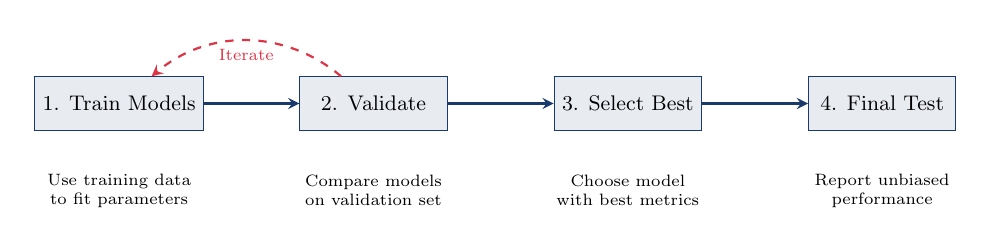
\begin{tikzpicture}[node distance=1.8cm, scale=0.85, transform shape]
        \tikzstyle{process} = [rectangle, minimum width=2.2cm, minimum height=0.8cm, text centered, draw=MainBlue, fill=MainBlue!10, font=\small]
        \tikzstyle{arrow} = [->, >=stealth, thick, MainBlue]

        % Nodes
        \node (train) [process] {1. Train Models};
        \node (validate) [process, right of=train, xshift=2cm] {2. Validate};
        \node (select) [process, right of=validate, xshift=2cm] {3. Select Best};
        \node (test) [process, right of=select, xshift=2cm] {4. Final Test};

        % Arrows
        \draw [arrow] (train) -- (validate);
        \draw [arrow] (validate) -- (select);
        \draw [arrow] (select) -- (test);

        % Feedback loop
        \draw [arrow, dashed, Crimson] (validate) to[bend right=40] node[below, font=\scriptsize] {Iterate} (train);

        % Labels below
        \node [below of=train, yshift=0.5cm, font=\scriptsize, text width=2.5cm, align=center] {Use training data\\to fit parameters};
        \node [below of=validate, yshift=0.5cm, font=\scriptsize, text width=2.5cm, align=center] {Compare models\\on validation set};
        \node [below of=select, yshift=0.5cm, font=\scriptsize, text width=2.5cm, align=center] {Choose model\\with best metrics};
        \node [below of=test, yshift=0.5cm, font=\scriptsize, text width=2.5cm, align=center] {Report unbiased\\performance};
    \end{tikzpicture}
    \end{center}

    \vspace{0.15cm}

    \begin{alertblock}{Critical Rule}
        \textbf{Never} use test set for model selection! This causes \textit{data leakage} and overly optimistic performance estimates.
    \end{alertblock}
\end{frame}

\begin{frame}{Real Data: Forecast Comparison}
    \begin{center}
        \includegraphics[width=0.95\textwidth, height=0.62\textheight, keepaspectratio]{real_data_forecast_comparison.pdf}
    \end{center}
    \vspace{-0.2cm}
    \begin{exampleblock}{Interpretation}
        \small Airline passengers data: Holt-Winters Multiplicative performs best for seasonal data.
    \end{exampleblock}
\end{frame}

\begin{frame}{Forecast Performance Across Datasets}
    \begin{center}
        \includegraphics[width=0.95\textwidth, height=0.68\textheight, keepaspectratio]{multiple_series_comparison.pdf}
    \end{center}
    \vspace{-0.2cm}
    \begin{exampleblock}{Interpretation}
        \small Different series require different models. Seasonal data needs seasonal methods.
    \end{exampleblock}
\end{frame}

%=============================================================================
% SECTION 5: MODELING SEASONALITY
%=============================================================================
\section{Modeling Seasonality}

\begin{frame}{Modeling Seasonality: Two Approaches}
    \begin{columns}[T]
        \begin{column}{0.48\textwidth}
            \textbf{1. Dummy Variables:}

            \vspace{0.1cm}
            $X_t = \mu + \sum_{j=1}^{s-1}\gamma_j D_{jt} + \varepsilon_t$

            \vspace{0.2cm}
            \begin{itemize}
                \item $D_{jt} = 1$ if $t$ in season $j$
                \item $s-1$ parameters
                \item Any seasonal pattern
            \end{itemize}
        \end{column}
        \begin{column}{0.48\textwidth}
            \textbf{2. Fourier Terms:}

            \vspace{0.1cm}
            $X_t = \mu + \sum_{k=1}^{K}[\alpha_k\sin(\cdot) + \beta_k\cos(\cdot)]$

            \vspace{0.2cm}
            \begin{itemize}
                \item Sinusoidal functions
                \item $2K$ parameters
                \item Smooth patterns
            \end{itemize}
        \end{column}
    \end{columns}

    \vspace{0.15cm}

    \begin{alertblock}{Trade-off}
        Dummies: any pattern, more parameters. Fourier: smooth, fewer parameters.
    \end{alertblock}
\end{frame}

\begin{frame}{Dummy Variables vs Fourier Terms}
    \begin{center}
        \includegraphics[width=0.95\textwidth, height=0.82\textheight, keepaspectratio]{seasonality_fourier_dummies.pdf}
    \end{center}
\end{frame}

\begin{frame}{Choosing Between Dummies and Fourier}
    \begin{center}
    \small
    \begin{tabular}{lcc}
        \toprule
        \textbf{Criterion} & \textbf{Dummies} & \textbf{Fourier} \\
        \midrule
        Parameters (monthly) & 11 & $2K$ (often 4--6) \\
        Seasonal pattern & Any shape & Smooth/sinusoidal \\
        Interpretation & Direct (month effects) & Frequency components \\
        High-frequency seasons & Many parameters & Efficient \\
        Multiple seasonality & Complex & Easy (add terms) \\
        \bottomrule
    \end{tabular}
    \end{center}

    \vspace{0.1cm}

    \begin{exampleblock}{Guidelines}
        \begin{itemize}
            \item Use \textbf{dummies}: irregular patterns, interpretable coefficients
            \item Use \textbf{Fourier}: smooth patterns, high-frequency seasonality, multiple periods
            \item \textbf{Fourier terms} are used in TBATS and Facebook Prophet
        \end{itemize}
    \end{exampleblock}
\end{frame}

%=============================================================================
% SECTION 6: HANDLING TREND AND SEASONALITY
%=============================================================================
\section{Handling Trend and Seasonality}

\begin{frame}{Why Remove Trend and Seasonality?}
    \textbf{Before modeling}, we often need to make series stationary:

    \vspace{0.15cm}

    \begin{columns}[T]
        \begin{column}{0.48\textwidth}
            \textbf{Reasons to detrend:}
            \begin{itemize}
                \item Stationarity requirement
                \item Focus on fluctuations
                \item Avoid spurious regression
                \item Enable valid inference
            \end{itemize}
        \end{column}
        \begin{column}{0.48\textwidth}
            \textbf{Reasons to deseasonalize:}
            \begin{itemize}
                \item Reveal underlying trend
                \item Compare across seasons
                \item Simplify modeling
                \item Focus on irregular component
            \end{itemize}
        \end{column}
    \end{columns}

    \vspace{0.2cm}

    \begin{alertblock}{Important}
        After modeling the detrended/deseasonalized series, we must \textbf{reverse the transformation} for forecasting.
    \end{alertblock}
\end{frame}

\begin{frame}{Trend Removal Methods}
    \begin{columns}[T]
        \column{0.55\textwidth}
        \begin{block}{Six Common Detrending Approaches}
            \begin{enumerate}
                \item \textbf{Differencing}: $\Delta X_t = X_t - X_{t-1}$
                \item \textbf{Linear regression}: $\hat{T}_t = \hat{\beta}_0 + \hat{\beta}_1 t$
                \item \textbf{Polynomial}: Higher-order polynomial
                \item \textbf{HP Filter}: Balance fit vs smoothness
                \item \textbf{Moving average}: $\hat{T}_t = MA_q(X_t)$
                \item \textbf{LOESS}: Local polynomial regression
            \end{enumerate}
        \end{block}
        \column{0.43\textwidth}
        \begin{exampleblock}{Choice Depends On}
            \begin{itemize}
                \item Nature of trend (deterministic vs stochastic)
                \item Purpose (forecasting vs analysis)
            \end{itemize}
        \end{exampleblock}
    \end{columns}
\end{frame}

\begin{frame}{Detrending Methods: Comparison}
    \begin{center}
        \includegraphics[width=0.95\textwidth, height=0.82\textheight, keepaspectratio]{detrending_methods.pdf}
    \end{center}
\end{frame}

\begin{frame}{Trend Estimation: Multiple Approaches}
    \begin{center}
        \includegraphics[width=0.95\textwidth, height=0.68\textheight, keepaspectratio]{trend_estimation_comparison.pdf}
    \end{center}
    \vspace{-0.2cm}
    \begin{exampleblock}{Interpretation}
        \small Different methods capture trend at varying levels of smoothness.
    \end{exampleblock}
\end{frame}

\begin{frame}{Seasonality Removal Methods}
    \begin{block}{Four Approaches to Remove Seasonality}
        \begin{enumerate}
            \item \textbf{Seasonal differencing}: $\Delta_s X_t = X_t - X_{t-s}$
            \item \textbf{Division} (multiplicative): $X_t^{adj} = X_t / \hat{S}_t$
            \item \textbf{Subtraction} (additive): $X_t^{adj} = X_t - \hat{S}_t$
            \item \textbf{X-13ARIMA-SEATS}: Government statistical method
        \end{enumerate}
    \end{block}

    \vspace{0.1cm}

    \begin{exampleblock}{Seasonal Period $s$}
        Monthly $\Rightarrow s=12$; Quarterly $\Rightarrow s=4$
    \end{exampleblock}
\end{frame}

\begin{frame}{Seasonal Adjustment: Visualization}
    \begin{center}
        \includegraphics[width=0.95\textwidth, height=0.82\textheight, keepaspectratio]{seasonal_adjustment.pdf}
    \end{center}
\end{frame}

\begin{frame}{Deterministic vs Stochastic Trend}
    \begin{columns}[T]
        \begin{column}{0.48\textwidth}
            \textbf{Deterministic Trend:}
            \[
                X_t = \beta_0 + \beta_1 t + \varepsilon_t
            \]
            \begin{itemize}
                \item Trend is a function of time
                \item Detrend by regression
                \item $\varepsilon_t$ is stationary
            \end{itemize}
        \end{column}
        \begin{column}{0.48\textwidth}
            \textbf{Stochastic Trend:}
            \[
                X_t = X_{t-1} + \varepsilon_t
            \]
            \begin{itemize}
                \item Random walk component
                \item Detrend by differencing
                \item $\Delta X_t$ is stationary
            \end{itemize}
        \end{column}
    \end{columns}

    \vspace{0.15cm}

    \begin{alertblock}{Wrong Method = Problems}
        \begin{itemize}
            \item Differencing deterministic trend $\Rightarrow$ over-differencing
            \item Regression on stochastic trend $\Rightarrow$ spurious regression
        \end{itemize}
    \end{alertblock}
\end{frame}

\begin{frame}{Example: Deterministic Trend}
    \begin{center}
        \includegraphics[width=0.95\textwidth, height=0.62\textheight, keepaspectratio]{deterministic_trend_example.pdf}
    \end{center}
    \vspace{-0.1cm}
    \begin{exampleblock}{Key}
        \small Use \textcolor{Crimson}{regression} to remove trend $\rightarrow$ residuals are stationary (ACF decays quickly).
    \end{exampleblock}
\end{frame}

\begin{frame}{Example: Stochastic Trend (Random Walk)}
    \begin{center}
        \includegraphics[width=0.95\textwidth, height=0.68\textheight, keepaspectratio]{stochastic_trend_example.pdf}
    \end{center}
    \vspace{-0.1cm}
    \begin{exampleblock}{Key}
        \small Use \textcolor{Crimson}{differencing} to remove trend $\rightarrow$ differences are stationary (white noise).
    \end{exampleblock}
\end{frame}

\begin{frame}{Side-by-Side Comparison}
    \begin{center}
        \includegraphics[width=0.95\textwidth, height=0.68\textheight, keepaspectratio]{trend_comparison_sidebyside.pdf}
    \end{center}
    \vspace{-0.2cm}
    \begin{alertblock}{Remember}
        \small Deterministic $\rightarrow$ regression. Stochastic $\rightarrow$ differencing.
    \end{alertblock}
\end{frame}

%=============================================================================
% SECTION 7: STOCHASTIC PROCESSES
%=============================================================================
\section{Stochastic Processes}

\begin{frame}{Stochastic Process: Definition}
    \begin{defn}[Stochastic Process]
        A \textbf{stochastic process} is a collection of random variables indexed by time:
        \[
            \{X_t(\omega) : t \in \mathcal{T}, \omega \in \Omega\}
        \]
        where $\Omega$ is the sample space of possible outcomes.
    \end{defn}

    \vspace{0.1cm}

    \begin{columns}[T]
        \column{0.48\textwidth}
        \begin{block}{Two Perspectives}
            \begin{itemize}
                \item \textbf{Fixed $\omega$}: A \textit{realization} $\{X_t(\omega)\}_{t \in \mathcal{T}}$
                \item \textbf{Fixed $t$}: A \textit{random variable} $X_t$
            \end{itemize}
        \end{block}
        \column{0.5\textwidth}
        \begin{exampleblock}{Key Insight}
            A time series we observe is \textbf{one realization} of the underlying stochastic process.
        \end{exampleblock}
    \end{columns}
\end{frame}

\begin{frame}{Stochastic Process: Visual Illustration}
    \begin{center}
        \includegraphics[width=0.95\textwidth, height=0.65\textheight, keepaspectratio]{ch1_def_stochastic.pdf}
    \end{center}
    \vspace{-0.2cm}
    \begin{exampleblock}{Interpretation}
        \small Each line is a different realization from the same stochastic process. We observe only one realization but want to understand the process.
    \end{exampleblock}
\end{frame}

\begin{frame}{Moments of a Stochastic Process}
    \begin{block}{First Two Moments Characterize Weak Properties}
        \textbf{Mean Function:} \quad $\mu_t = \E[X_t]$

        \vspace{0.15cm}

        \textbf{Autocovariance Function (ACVF):}
        \[
            \gamma(t, s) = \Cov(X_t, X_s) = \E[(X_t - \mu_t)(X_s - \mu_s)]
        \]

        \textbf{Autocorrelation Function (ACF):}
        \[
            \rho(t, s) = \frac{\gamma(t, s)}{\sqrt{\Var(X_t) \cdot \Var(X_s)}}
        \]
    \end{block}

    \begin{exampleblock}{Properties}
        $\rho(t, s) \in [-1, 1]$ and $\rho(t, t) = 1$
    \end{exampleblock}
\end{frame}

%=============================================================================
% SECTION 4: STATIONARITY
%=============================================================================
\section{Stationarity}

\begin{frame}{Why Stationarity Matters}
    \textbf{Stationarity} is a fundamental assumption for time series analysis:

    \vspace{0.15cm}

    \begin{columns}[T]
        \begin{column}{0.48\textwidth}
            \textbf{\textcolor{Crimson}{Without Stationarity:}}
            \begin{itemize}
                \item Mean, variance change over time
                \item Past may not predict future
                \item Standard methods fail
                \item Spurious correlations
            \end{itemize}
        \end{column}
        \begin{column}{0.48\textwidth}
            \textbf{\textcolor{Forest}{With Stationarity:}}
            \begin{itemize}
                \item Statistical properties constant
                \item Can estimate from one realization
                \item Valid inference possible
                \item Models are meaningful
            \end{itemize}
        \end{column}
    \end{columns}

    \vspace{0.2cm}

    \begin{alertblock}{Key Principle}
        Most time series models (ARMA, ARIMA, etc.) require stationarity. Non-stationary series must be transformed (e.g., differencing) before modeling.
    \end{alertblock}
\end{frame}

\begin{frame}{Stationary vs Non-Stationary: Visual Comparison}
    \vspace{-0.3cm}
    \begin{center}
        \includegraphics[width=0.95\textwidth, height=0.62\textheight, keepaspectratio]{ch1_stationarity.pdf}
    \end{center}
    \vspace{-0.2cm}
    {\footnotesize
    \begin{itemize}
        \item \textbf{Stationary}: Constant mean and variance -- fluctuates around a fixed level
        \item \textbf{Non-stationary}: Mean and/or variance change over time
        \item Visual inspection is the first step; formal tests (ADF, KPSS) confirm
    \end{itemize}
    }
\end{frame}

\begin{frame}{Strict Stationarity}
    \begin{defn}[Strict (Strong) Stationarity]
        A process $\{X_t\}$ is \textbf{strictly stationary} if for all $k$, all $t_1, \ldots, t_k$, and all $h$:
        \[
            (X_{t_1}, X_{t_2}, \ldots, X_{t_k}) \stackrel{d}{=} (X_{t_1+h}, X_{t_2+h}, \ldots, X_{t_k+h})
        \]
    \end{defn}

    \begin{columns}[T]
        \column{0.55\textwidth}
        \begin{block}{Implications}
            \begin{itemize}
                \item All marginal distributions $F_{X_t}(x)$ identical
                \item $\E[X_t] = \mu$ (constant mean)
                \item $\Var(X_t) = \sigma^2$ (constant variance)
                \item Joint distributions depend only on lag
            \end{itemize}
        \end{block}
        \column{0.43\textwidth}
        \begin{alertblock}{Note}
            Strict stationarity is a strong condition, often impractical to verify.
        \end{alertblock}
    \end{columns}
\end{frame}

\begin{frame}{Strict Stationarity: Visual Illustration}
    \begin{center}
        \includegraphics[width=0.95\textwidth, height=0.65\textheight, keepaspectratio]{ch1_def_strict_stationarity.pdf}
    \end{center}
    \vspace{-0.2cm}
    \begin{exampleblock}{Interpretation}
        \small Stationary: any two windows have the same joint distribution. Non-stationary: distribution changes over time.
    \end{exampleblock}
\end{frame}

\begin{frame}{Weak (Covariance) Stationarity}
    \begin{defn}[Weak Stationarity]
        A process $\{X_t\}$ is \textbf{weakly stationary} (or covariance stationary) if:
        \begin{enumerate}
            \item $\E[X_t] = \mu$ \quad (constant mean)
            \item $\Var(X_t) = \sigma^2 < \infty$ \quad (constant, finite variance)
            \item $\Cov(X_t, X_{t+h}) = \gamma(h)$ \quad (covariance depends only on lag $h$)
        \end{enumerate}
    \end{defn}

    \vspace{0.15cm}

    \textbf{Key property:} Autocovariance is a function of lag only:
    \begin{equation}
        \gamma(h) = \Cov(X_t, X_{t+h}) = \E[(X_t - \mu)(X_{t+h} - \mu)]
    \end{equation}

    \textbf{Autocorrelation function:}
    \begin{equation}
        \rho(h) = \frac{\gamma(h)}{\gamma(0)} = \frac{\Cov(X_t, X_{t+h})}{\Var(X_t)}
    \end{equation}

    Note: $\rho(0) = 1$ and $\rho(h) = \rho(-h)$ (symmetry)
\end{frame}

\begin{frame}{Weak Stationarity: Visual Illustration}
    \begin{center}
        \includegraphics[width=0.95\textwidth, height=0.65\textheight, keepaspectratio]{ch1_def_weak_stationarity.pdf}
    \end{center}
    \vspace{-0.2cm}
    \begin{exampleblock}{Interpretation}
        \small Left: constant mean and variance. Right: autocovariance depends only on lag $h$, not time $t$.
    \end{exampleblock}
\end{frame}

\begin{frame}{Properties of the Autocovariance Function}
    \begin{block}{ACVF Properties for Weakly Stationary Process}
        The ACVF $\gamma(h)$ satisfies:
        \begin{enumerate}
            \item \textbf{Symmetry:} $\gamma(h) = \gamma(-h)$
            \item \textbf{Maximum at zero:} $|\gamma(h)| \leq \gamma(0)$
            \item \textbf{Non-negative definiteness}
        \end{enumerate}
    \end{block}

    \vspace{0.2cm}

    \begin{alertblock}{Implication}
        Not every function can be an autocovariance function.
    \end{alertblock}
\end{frame}

%=============================================================================
% SECTION 5: WHITE NOISE AND RANDOM WALK
%=============================================================================
\section{White Noise and Random Walk}

\begin{frame}{White Noise Process}
    \begin{defn}[White Noise]
        A process $\{\varepsilon_t\}$ is \textbf{white noise}, denoted $\varepsilon_t \sim WN(0, \sigma^2)$, if:
        \begin{enumerate}
            \item $\E[\varepsilon_t] = 0$ for all $t$
            \item $\Var(\varepsilon_t) = \sigma^2$ for all $t$
            \item $\Cov(\varepsilon_t, \varepsilon_s) = 0$ for $t \neq s$
        \end{enumerate}
    \end{defn}

    \begin{columns}[T]
        \column{0.45\textwidth}
        \begin{block}{ACF of White Noise}
            \[
                \rho(h) = \begin{cases}
                    1 & \text{if } h = 0 \\
                    0 & \text{if } h \neq 0
                \end{cases}
            \]
        \end{block}
        \column{0.53\textwidth}
        \begin{exampleblock}{Types}
            \begin{itemize}
                \item \textbf{Weak}: Uncorrelated
                \item \textbf{Strong}: i.i.d.
                \item \textbf{Gaussian}: $\varepsilon_t \stackrel{iid}{\sim} N(0, \sigma^2)$
            \end{itemize}
        \end{exampleblock}
    \end{columns}
\end{frame}

\begin{frame}{White Noise vs Random Walk: Comparison}
    \vspace{-0.3cm}
    \begin{center}
        \includegraphics[width=0.95\textwidth, height=0.62\textheight, keepaspectratio]{ch1_wn_rw.pdf}
    \end{center}
    \vspace{-0.2cm}
    {\footnotesize
    \begin{itemize}
        \item \textbf{White noise}: Fluctuates around zero -- stationary, constant variance
        \item \textbf{Random walk}: Cumulative sum of white noise -- wanders away, non-stationary
        \item Random walk is the simplest non-stationary process (unit root)
    \end{itemize}
    }
\end{frame}

\begin{frame}{White Noise: Visual Illustration}
    \begin{center}
        \includegraphics[width=0.95\textwidth, height=0.65\textheight, keepaspectratio]{ch1_def_white_noise.pdf}
    \end{center}
    \vspace{-0.2cm}
    \begin{exampleblock}{Interpretation}
        \small Left: white noise fluctuates around zero with constant variance. Right: ACF shows no autocorrelation (all zero after lag 0).
    \end{exampleblock}
\end{frame}

\begin{frame}{Random Walk Process}
    \begin{block}{Definition}
        $X_t = X_{t-1} + \varepsilon_t$ where $\varepsilon_t \sim WN(0, \sigma^2)$, $X_0 = 0$

        \textbf{Explicit form:} $X_t = \sum_{i=1}^{t} \varepsilon_i$
    \end{block}

    \begin{columns}[T]
        \column{0.5\textwidth}
        \begin{exampleblock}{Properties}
            \begin{itemize}
                \item $\E[X_t] = 0$ (constant mean)
                \item $\Var(X_t) = t\sigma^2$ (grows with time!)
                \item $\Cov(X_t, X_s) = \min(t, s) \cdot \sigma^2$
            \end{itemize}
        \end{exampleblock}
        \column{0.48\textwidth}
        \begin{alertblock}{Non-Stationary!}
            Random walk is \textbf{not stationary} because variance depends on $t$.
        \end{alertblock}
    \end{columns}
\end{frame}

\begin{frame}{Random Walk: Visualization}
    \begin{center}
        \includegraphics[width=0.95\textwidth, height=0.65\textheight, keepaspectratio]{random_walk.pdf}
    \end{center}
    \vspace{-0.2cm}
    \begin{exampleblock}{Interpretation}
        \small \textbf{Left:} Multiple paths diverge over time. \textbf{Right:} Variance grows linearly: $\Var(X_t) = t\sigma^2$.
    \end{exampleblock}
\end{frame}

\begin{frame}{Stationary vs Non-Stationary: Comparison}
    \begin{center}
        \includegraphics[width=0.95\textwidth, height=0.65\textheight, keepaspectratio]{rw_vs_stationary.pdf}
    \end{center}
    \vspace{-0.2cm}
    \begin{exampleblock}{Key Diagnostic}
        \small ACF of stationary process decays quickly; ACF of random walk decays very slowly.
    \end{exampleblock}
\end{frame}

%=============================================================================
% SECTION 6: ACF AND PACF
%=============================================================================
\section{Autocorrelation Functions}

\begin{frame}{Sample Autocorrelation Function}
    \begin{block}{Sample ACF at Lag $h$}
        \begin{equation}
            \hat{\rho}(h) = \frac{\sum_{t=1}^{T-h}(x_t - \bar{x})(x_{t+h} - \bar{x})}{\sum_{t=1}^{T}(x_t - \bar{x})^2}
        \end{equation}
    \end{block}

    \begin{columns}[T]
        \column{0.45\textwidth}
        \begin{exampleblock}{Properties}
            \begin{itemize}
                \item $\hat{\rho}(0) = 1$ always
                \item $|\hat{\rho}(h)| \leq 1$
            \end{itemize}
        \end{exampleblock}
        \column{0.53\textwidth}
        \begin{alertblock}{Significance Test}
            Under white noise: $\hat{\rho}(h) \approx N(0, 1/T)$

            \textbf{95\% bounds:} $\pm 1.96/\sqrt{T}$
        \end{alertblock}
    \end{columns}
\end{frame}

\begin{frame}{ACF Patterns for Different Processes}
    \vspace{-0.3cm}
    \begin{center}
        \includegraphics[width=0.95\textwidth, height=0.62\textheight, keepaspectratio]{ch1_acf_examples.pdf}
    \end{center}
    \vspace{-0.2cm}
    {\footnotesize
    \begin{itemize}
        \item \textbf{White noise}: ACF drops to zero immediately (no dependence)
        \item \textbf{AR(1)}: ACF decays exponentially -- indicates autoregressive structure
        \item \textbf{Seasonal}: ACF shows spikes at seasonal lags (e.g., 12, 24 for monthly)
        \item \textbf{Random walk}: ACF decays very slowly -- sign of non-stationarity
    \end{itemize}
    }
\end{frame}

\begin{frame}{Partial Autocorrelation Function (PACF)}
    \begin{block}{Definition}
        \textbf{PACF} $\phi_{hh}$: Correlation between $X_t$ and $X_{t+h}$ after removing the linear effect of $X_{t+1}, \ldots, X_{t+h-1}$.
    \end{block}

    \begin{columns}[T]
        \column{0.48\textwidth}
        \begin{exampleblock}{Interpretation}
            \begin{itemize}
                \item $\phi_{11} = \rho(1)$ (same as ACF at lag 1)
                \item $\phi_{22}$: correlation controlling for $X_{t+1}$
                \item Measures \textit{direct} dependence
            \end{itemize}
        \end{exampleblock}
        \column{0.5\textwidth}
        \begin{alertblock}{Key Application}
            \begin{itemize}
                \item AR($p$): PACF \textbf{cuts off} after lag $p$
                \item MA($q$): ACF \textbf{cuts off} after lag $q$
            \end{itemize}
        \end{alertblock}
    \end{columns}
\end{frame}

\begin{frame}{ACF and PACF Patterns}
    \begin{center}
        \includegraphics[width=0.95\textwidth, height=0.82\textheight, keepaspectratio]{acf_pacf_examples.pdf}
    \end{center}
\end{frame}

\begin{frame}{Theoretical ACF for AR(1)}
    \begin{center}
        \includegraphics[width=0.95\textwidth, height=0.68\textheight, keepaspectratio]{acf_theoretical.pdf}
    \end{center}
    \vspace{-0.2cm}
    \begin{exampleblock}{Interpretation}
        \small For AR(1): $X_t = \phi X_{t-1} + \varepsilon_t$, the theoretical ACF is $\rho(h) = \phi^h$.
    \end{exampleblock}
\end{frame}

%=============================================================================
% SECTION 7: LAG OPERATOR AND DIFFERENCING
%=============================================================================
\section{Lag Operator and Differencing}

\begin{frame}{The Lag Operator}
    \begin{defn}[Lag Operator]
        The \textbf{lag operator} (or backshift operator) $L$ is defined by:
        \[
            LX_t = X_{t-1}
        \]
    \end{defn}

    \begin{columns}[T]
        \column{0.48\textwidth}
        \begin{block}{Properties}
            \begin{itemize}
                \item $L^k X_t = X_{t-k}$ (lag by $k$ periods)
                \item $L^0 = I$ (identity)
                \item $(1 - \phi L)X_t = X_t - \phi X_{t-1}$
            \end{itemize}
        \end{block}
        \column{0.5\textwidth}
        \begin{exampleblock}{Examples}
            \begin{itemize}
                \item AR(1): $(1 - \phi L)X_t = \varepsilon_t$
                \item MA(1): $X_t = (1 + \theta L)\varepsilon_t$
                \item AR($p$): $\phi(L)X_t = \varepsilon_t$
            \end{itemize}
        \end{exampleblock}
    \end{columns}
\end{frame}

\begin{frame}{Lag Operator: Visual Illustration}
    \begin{center}
        \includegraphics[width=0.95\textwidth, height=0.65\textheight, keepaspectratio]{ch1_def_lag_operator.pdf}
    \end{center}
    \vspace{-0.2cm}
    \begin{exampleblock}{Interpretation}
        \small The lag operator $L$ shifts every observation back by one time period: $LX_t = X_{t-1}$.
    \end{exampleblock}
\end{frame}

\begin{frame}{Differencing}
    \begin{block}{First Difference}
        $\Delta X_t = X_t - X_{t-1} = (1 - L)X_t$
    \end{block}

    \begin{columns}[T]
        \column{0.48\textwidth}
        \begin{exampleblock}{Why Difference?}
            \begin{itemize}
                \item Removes trend and unit root
                \item Random walk: $\Delta X_t = \varepsilon_t$ (white noise)
            \end{itemize}
        \end{exampleblock}
        \column{0.5\textwidth}
        \begin{block}{Integrated Process}
            $X_t \sim I(d)$ if $\Delta^d X_t$ is stationary
            \begin{itemize}
                \item $I(0)$: Stationary (no differencing)
                \item $I(1)$: One difference needed
                \item $I(2)$: Two differences needed
            \end{itemize}
        \end{block}
    \end{columns}
\end{frame}

\begin{frame}{Effect of Differencing: S\&P 500}
    \begin{center}
        \includegraphics[width=0.95\textwidth, height=0.82\textheight, keepaspectratio]{differencing_effect.pdf}
    \end{center}
\end{frame}

%=============================================================================
% SECTION 8: TESTING FOR STATIONARITY
%=============================================================================
\section{Testing for Stationarity}

\begin{frame}{Augmented Dickey-Fuller (ADF) Test}
    \begin{block}{Model}
        $\Delta X_t = \alpha + \gamma X_{t-1} + \sum_{i=1}^{p} \delta_i \Delta X_{t-i} + \varepsilon_t$
    \end{block}

    \vspace{0.1cm}

    \begin{columns}[T]
        \begin{column}{0.48\textwidth}
            \begin{exampleblock}{Hypotheses}
                \begin{itemize}
                    \item $H_0$: $\gamma = 0$ (unit root)
                    \item $H_1$: $\gamma < 0$ (stationary)
                \end{itemize}
            \end{exampleblock}
        \end{column}
        \begin{column}{0.48\textwidth}
            \begin{block}{Test Statistic}
                \[
                    \tau = \frac{\hat{\gamma}}{SE(\hat{\gamma})}
                \]
            \end{block}
        \end{column}
    \end{columns}

    \vspace{0.1cm}

    \begin{alertblock}{Decision Rule}
        $\tau <$ critical value $\Rightarrow$ Reject $H_0$ $\Rightarrow$ \textcolor{Forest}{Stationary} \\
        $\tau \geq$ critical value $\Rightarrow$ \textcolor{Crimson}{Non-stationary}
    \end{alertblock}
\end{frame}

\begin{frame}{KPSS Test}
    \begin{block}{Model}
        $X_t = \xi t + r_t + \varepsilon_t$ where $r_t = r_{t-1} + u_t$
    \end{block}

    \vspace{0.1cm}

    \begin{columns}[T]
        \begin{column}{0.48\textwidth}
            \begin{exampleblock}{Hypotheses (opposite of ADF)}
                \begin{itemize}
                    \item $H_0$: $\sigma_u^2 = 0$ (stationary)
                    \item $H_1$: $\sigma_u^2 > 0$ (unit root)
                \end{itemize}
            \end{exampleblock}
        \end{column}
        \begin{column}{0.48\textwidth}
            \begin{block}{Test Statistic}
                \[
                    LM = \frac{\sum_{t=1}^{T} S_t^2}{T^2 \hat{\sigma}^2}
                \]
                {\small where $S_t = \sum_{i=1}^{t} \hat{e}_i$}
            \end{block}
        \end{column}
    \end{columns}

    \vspace{0.1cm}

    \begin{alertblock}{Decision Rule}
        $LM >$ critical value $\Rightarrow$ Reject $H_0$ $\Rightarrow$ \textcolor{Crimson}{Non-stationary} \\
        $LM \leq$ critical value $\Rightarrow$ \textcolor{Forest}{Stationary}
    \end{alertblock}
\end{frame}

\begin{frame}{Using ADF and KPSS Together}
    \begin{block}{Confirmatory Testing for Robust Conclusions}
        \begin{center}
        \small
        \begin{tabular}{lccl}
            \toprule
            \textbf{ADF} & \textbf{KPSS} & \textbf{Conclusion} \\
            \midrule
            Reject $H_0$ & Fail to reject $H_0$ & \textcolor{Forest}{Stationary} \\
            Fail to reject $H_0$ & Reject $H_0$ & \textcolor{Crimson}{Unit Root} \\
            Reject $H_0$ & Reject $H_0$ & Inconclusive \\
            Fail to reject $H_0$ & Fail to reject $H_0$ & Inconclusive \\
            \bottomrule
        \end{tabular}
        \end{center}
    \end{block}

    \begin{exampleblock}{Recommended Workflow}
        \begin{enumerate}
            \item Run ADF test (null = unit root)
            \item Run KPSS test (null = stationary)
            \item If results agree, proceed with confidence
            \item If inconclusive, consider alternative tests (PP, DF-GLS)
        \end{enumerate}
    \end{exampleblock}
\end{frame}

\begin{frame}{ADF Test: Visualization with S\&P 500}
    \begin{center}
        \includegraphics[width=0.95\textwidth, height=0.82\textheight, keepaspectratio]{adf_test_visualization.pdf}
    \end{center}
\end{frame}

%=============================================================================
% SECTION 9: REAL DATA APPLICATION
%=============================================================================
\section{Financial Data Application}

\begin{frame}{S\&P 500 Analysis: Overview}
    \begin{center}
        \includegraphics[width=0.95\textwidth, height=0.82\textheight, keepaspectratio]{sp500_analysis.pdf}
    \end{center}
\end{frame}

\begin{frame}{Stylized Facts of Financial Returns}
    \begin{center}
        \includegraphics[width=0.95\textwidth, height=0.48\textheight, keepaspectratio]{returns_distribution.pdf}
    \end{center}
    \vspace{-0.1cm}
    \begin{columns}[T]
        \begin{column}{0.48\textwidth}
            \textbf{Observed properties:}
            \begin{itemize}
                \item Negative skewness (left tail)
                \item Excess kurtosis ($\gg 3$)
                \item Heavy tails (fat tails)
            \end{itemize}
        \end{column}
        \begin{column}{0.48\textwidth}
            \textbf{Implications:}
            \begin{itemize}
                \item Normal distribution inadequate
                \item Extreme events more likely
                \item Need Student-t or similar
            \end{itemize}
        \end{column}
    \end{columns}
\end{frame}

\begin{frame}{Volatility Clustering}
    \begin{center}
        \includegraphics[width=0.95\textwidth, height=0.55\textheight, keepaspectratio]{volatility_clustering.pdf}
    \end{center}
    \vspace{-0.1cm}
    \begin{alertblock}{Stylized Fact}
        Large returns (positive or negative) tend to be followed by large returns. This \textbf{volatility clustering} motivates ARCH/GARCH models (future chapters).
    \end{alertblock}
\end{frame}

%=============================================================================
% SECTION 10: SUMMARY
%=============================================================================
\section{Summary}

\begin{frame}{Key Takeaways}
    \begin{block}{Summary}
    \small
    \begin{enumerate}
        \item \textbf{Time series} = observations indexed by time with temporal dependence
        \item \textbf{Decomposition}: Additive $X_t = T_t + S_t + \varepsilon_t$ or Multiplicative
        \item \textbf{Exponential Smoothing}: SES (level), Holt (trend), Holt-Winters (seasonal)
        \item \textbf{Forecast Evaluation}: MAE, RMSE, MAPE; use train/validation/test splits
        \item \textbf{Seasonality Modeling}: Dummy variables (any pattern) or Fourier terms (smooth)
        \item \textbf{Trend Handling}: Differencing (stochastic) or regression (deterministic)
        \item \textbf{Stationarity}: Mean, variance, autocovariance constant over time
        \item \textbf{ACF/PACF}: Essential for identifying dependence structure
        \item \textbf{Unit root tests}: ADF ($H_0$: unit root) vs KPSS ($H_0$: stationary)
    \end{enumerate}
    \end{block}
\end{frame}

\begin{frame}{Important Formulas I}
    \begin{block}{Decomposition}
        Additive: $X_t = T_t + S_t + \varepsilon_t$ \quad Multiplicative: $X_t = T_t \times S_t \times \varepsilon_t$
    \end{block}

    \begin{block}{Simple Exponential Smoothing (SES)}
        $\hat{X}_{t+1|t} = \alpha X_t + (1-\alpha)\hat{X}_{t|t-1}$ \quad where $\alpha \in (0,1)$
    \end{block}

    \begin{block}{Holt's Linear Trend}
        $\ell_t = \alpha X_t + (1-\alpha)(\ell_{t-1} + b_{t-1})$ \quad $b_t = \beta^*(\ell_t - \ell_{t-1}) + (1-\beta^*)b_{t-1}$
    \end{block}

    \begin{block}{Holt-Winters Additive}
        $\ell_t = \alpha(X_t - S_{t-s}) + (1-\alpha)(\ell_{t-1} + b_{t-1})$ \quad $S_t = \gamma(X_t - \ell_t) + (1-\gamma)S_{t-s}$
    \end{block}
\end{frame}

\begin{frame}{Important Formulas II}
    \begin{block}{Moving Average (Trend Estimation)}
        $\hat{T}_t = \frac{1}{2q+1}\sum_{j=-q}^{q} X_{t+j}$
    \end{block}

    \begin{block}{Autocovariance and Autocorrelation}
        $\gamma(h) = \Cov(X_t, X_{t+h})$ \qquad $\rho(h) = \frac{\gamma(h)}{\gamma(0)}$
    \end{block}

    \begin{block}{Random Walk}
        $X_t = X_{t-1} + \varepsilon_t$ \quad $\Rightarrow$ \quad $\Var(X_t) = t\sigma^2$ (non-stationary)
    \end{block}

    \begin{block}{Differencing}
        $\Delta X_t = (1-L)X_t = X_t - X_{t-1}$
    \end{block}
\end{frame}

\begin{frame}{Next Chapter Preview}
    \begin{block}{Chapter 2: ARMA Models}
        \begin{itemize}
            \item Autoregressive (AR) models
            \item Moving Average (MA) models
            \item Combined ARMA models
            \item Model identification using ACF/PACF
            \item Parameter estimation
            \item Model diagnostics
            \item Forecasting
        \end{itemize}
    \end{block}
\end{frame}

%=============================================================================
% SECTION: QUIZ
%=============================================================================
\section{Quiz}

\begin{frame}{Quiz Question 1}
    \begin{alertblock}{Question}
        A time series $Y_t$ shows upward movement over years plus repeating patterns each quarter. Which components are present?
    \end{alertblock}

    \vspace{0.3cm}

    \begin{enumerate}[(A)]
        \item Trend only
        \item Seasonality only
        \item Trend and Seasonality
        \item Random noise only
    \end{enumerate}
\end{frame}

\begin{frame}{Quiz Question 1: Answer}
    \begin{center}
        \includegraphics[width=0.95\textwidth, height=0.58\textheight, keepaspectratio]{ch1_quiz1_components.pdf}
    \end{center}
    \vspace{-0.2cm}
    \begin{exampleblock}{Correct Answer: (C) Trend and Seasonality}
        Upward movement = Trend; Quarterly patterns = Seasonality (s=4)
    \end{exampleblock}
\end{frame}

\begin{frame}{Quiz Question 2}
    \begin{alertblock}{Question}
        Which of the following is a characteristic of a stationary time series?
    \end{alertblock}

    \vspace{0.3cm}

    \begin{enumerate}[(A)]
        \item Mean changes over time
        \item Variance increases with time
        \item Constant mean and variance over time
        \item Contains a trend component
    \end{enumerate}
\end{frame}

\begin{frame}{Quiz Question 2: Answer}
    \begin{center}
        \includegraphics[width=0.95\textwidth, height=0.58\textheight, keepaspectratio]{ch1_quiz2_stationarity.pdf}
    \end{center}
    \vspace{-0.2cm}
    \begin{exampleblock}{Correct Answer: (C) Constant mean and variance over time}
        Stationarity requires: constant mean, constant variance, and autocovariance depends only on lag.
    \end{exampleblock}
\end{frame}

\begin{frame}{Quiz Question 3}
    \begin{alertblock}{Question}
        For a white noise process, what does the ACF look like at lags $k > 0$?
    \end{alertblock}

    \vspace{0.3cm}

    \begin{enumerate}[(A)]
        \item Exponential decay
        \item All values significant and positive
        \item All values approximately zero (within confidence bands)
        \item Alternating positive and negative
    \end{enumerate}
\end{frame}

\begin{frame}{Quiz Question 3: Answer}
    \begin{center}
        \includegraphics[width=0.95\textwidth, height=0.58\textheight, keepaspectratio]{ch1_quiz3_acf.pdf}
    \end{center}
    \vspace{-0.2cm}
    \begin{exampleblock}{Correct Answer: (C) Approximately zero within confidence bands}
        White noise has no autocorrelation: $\rho_k = 0$ for all $k \neq 0$.
    \end{exampleblock}
\end{frame}

\begin{frame}{Quiz Question 4}
    \begin{alertblock}{Question}
        What is the key difference between white noise and a random walk?
    \end{alertblock}

    \vspace{0.3cm}

    \begin{enumerate}[(A)]
        \item White noise has a trend, random walk doesn't
        \item Random walk is the cumulative sum of white noise
        \item Both are stationary processes
        \item White noise has higher variance
    \end{enumerate}
\end{frame}

\begin{frame}{Quiz Question 4: Answer}
    \begin{center}
        \includegraphics[width=0.95\textwidth, height=0.58\textheight, keepaspectratio]{ch1_quiz4_wn_rw.pdf}
    \end{center}
    \vspace{-0.2cm}
    \begin{exampleblock}{Correct Answer: (B) Random walk = cumulative sum of white noise}
        $Y_t = Y_{t-1} + \varepsilon_t = \sum_{i=1}^t \varepsilon_i$ where $\varepsilon_t$ is white noise.
    \end{exampleblock}
\end{frame}

\begin{frame}{Quiz Question 5}
    \begin{alertblock}{Question}
        Which forecast error metric is most sensitive to large errors (outliers)?
    \end{alertblock}

    \vspace{0.3cm}

    \begin{enumerate}[(A)]
        \item MAE (Mean Absolute Error)
        \item RMSE (Root Mean Squared Error)
        \item MAPE (Mean Absolute Percentage Error)
        \item All are equally sensitive
    \end{enumerate}
\end{frame}

\begin{frame}{Quiz Question 5: Answer}
    \begin{center}
        \includegraphics[width=0.95\textwidth, height=0.58\textheight, keepaspectratio]{ch1_quiz5_forecast_errors.pdf}
    \end{center}
    \vspace{-0.2cm}
    \begin{exampleblock}{Correct Answer: (B) RMSE}
        RMSE squares errors, so large errors have disproportionate impact: $\sqrt{\frac{1}{n}\sum e_t^2}$
    \end{exampleblock}
\end{frame}

\begin{frame}{Quiz Question 6}
    \begin{alertblock}{Question}
        When should you use multiplicative decomposition instead of additive?
    \end{alertblock}

    \vspace{0.3cm}

    \begin{enumerate}[(A)]
        \item When the series has no trend
        \item When seasonal amplitude is constant
        \item When seasonal amplitude grows with the level of the series
        \item When the series is stationary
    \end{enumerate}
\end{frame}

\begin{frame}{Quiz Question 6: Answer}
    \begin{center}
        \includegraphics[width=0.95\textwidth, height=0.58\textheight, keepaspectratio]{ch1_quiz6_decomposition.pdf}
    \end{center}
    \vspace{-0.2cm}
    \begin{exampleblock}{Correct Answer: (C) Seasonal amplitude grows with level}
        Multiplicative: $Y_t = T_t \times S_t \times \varepsilon_t$ --- seasonal swings proportional to trend.
    \end{exampleblock}
\end{frame}

\begin{frame}{References}
    \footnotesize
    \begin{thebibliography}{99}
        \bibitem{hyndman2021} Hyndman, R.J., \& Athanasopoulos, G. (2021). \textit{Forecasting: Principles and Practice}. 3rd ed., OTexts.

        \bibitem{hamilton1994} Hamilton, J.D. (1994). \textit{Time Series Analysis}. Princeton University Press.

        \bibitem{box2015} Box, G.E.P., Jenkins, G.M., Reinsel, G.C., \& Ljung, G.M. (2015). \textit{Time Series Analysis: Forecasting and Control}. 5th ed., Wiley.

        \bibitem{tsay2010} Tsay, R.S. (2010). \textit{Analysis of Financial Time Series}. 3rd ed., Wiley.

        \bibitem{cleveland1990} Cleveland, R.B., Cleveland, W.S., McRae, J.E., \& Terpenning, I. (1990). STL: A Seasonal-Trend Decomposition. \textit{Journal of Official Statistics}, 6(1), 3-73.
    \end{thebibliography}
\end{frame}

%=============================================================================
% DATA SOURCES
%=============================================================================
\begin{frame}{Data Sources}
    \begin{block}{Real Data Used in This Chapter}
        \begin{itemize}
            \item \textbf{Airline Passengers}: Box-Jenkins classic dataset, 1949--1960
            \item \textbf{S\&P 500}: Yahoo Finance (SPY), historical data
            \item \textbf{Sunspots}: Statsmodels dataset, monthly observations
        \end{itemize}
    \end{block}

    \begin{block}{Software \& Tools}
        \begin{itemize}
            \item \textbf{Python}: statsmodels, pandas, matplotlib, yfinance
            \item \textbf{R}: forecast, tseries packages
            \item \textbf{Data Sources}: Yahoo Finance, FRED Economic Data
        \end{itemize}
    \end{block}
\end{frame}

\begin{frame}{}
    \centering
    \Huge\textcolor{MainBlue}{Thank You!}

    \vspace{1cm}

    \Large Questions?

    \vspace{0.8cm}

    \normalsize
    \textit{Charts generated using Python (statsmodels, matplotlib)}

    \vspace{0.3cm}

    Course materials available at: \url{https://github.com/danpele/Time-Series-Analysis}
\end{frame}

\end{document}
